%************************************************
\chapter{Objectives and Analysis}\label{ch:objectives}
%************************************************

In this chapter we describe the project objectives, and the methodology followed during its development. We continue then describing the privacy-preserving attribute based credentials and the ecosystem surrounding it, from the P2ABCE's perspective, as it is the starting point of our project. We finish with an introduction to all the technologies involved in our development, from P2ABCE's code, to how smart cards work.

\section{Project description}\label{objectives:section}

The purpose of this project is the integration of IBM's privacy preserving solution, Idemix, in the environment of the Internet of Things. The objective is to design a general solution for the existing IoT devices and systems, without compromising any feature of Idemix, and provide a working PoC in a real IoT environment, even though it isn't the most constrained scenario. The project is aimed to be used in privacy-preserving environments, providing security for IoT, controlling what data is being disclosed and to whom.

In a smart city project, citizens' data can be privatized and at the same time continue to offer the benefits of the sensors around. Authorized personnel can disclose the information when required, like fire-fighters accessing a building's sensors to check how many people there are and what conditions they are in, in case of an emergency; but keep such invasive data private to other non-critical services, for example, only giving a proof that there are people in a floor of the building, to activate or deactivate the air-conditioning system.

\hfil


We will divide the project in various objectives:

The main objective of this thesis is to integrate IBM’s privacy-preserving Attribute Based System in the IoT environment. The idea is to enable IoT constrained devices to act as a autonomous entities that can authenticate and prove their attributes against a verifier entity using the Idemix protocol, thereby, allowing a privacy-preserving IdM solution for IoT.

This general objective, can be split in 6 main subobjectives: 



\begin{enumerate}
	\item Study of the Idemix ecosystem
	
	Study the state of the art of Idemix and the IoT, analysing the related projects and papers with similar approaches. Once we know as much as we can from the existing ecosystem, we will be able to deliver the most fitting solution to our project.
	
	\item Design of the IoT+Idemix solution
	
	A formal description of the IoT architecture that will that will allow to integrate Idemix in IoT scenarios.
	
	
	\item Implementation of a functional PoC
	
	\subitem Software objectives
	
	A maintainable, structured and extensible solution, from the IoT and original project perspectives, that is, the IoT solution must be interoperable with other non-IoT solutions, now and in the future, given new IoT systems or changes in the cryptographic protocols.
	
	\subitem Hardware objectives
	
	The implemented software needs to be optimized to be deployable in IoT devices as constrained as possible, and consider the multiple IoT platforms in existence.
	
	
	\item Validation of the PoC
	
	Deploy a \ac{PoC} in a real scenario, without the need of simulators, checking that it works as expected.
	
	\item Evaluation of performance
	
	This evaluation will allow to validate the feasibility of our solution and its implementation.
	
	\item Integrate the IoT+Idemix as a security solution for other projects
	
	The IoT+Idemix project is a solution for the privacy threads in the IoT environment, and does not work on its own, but as part of other projects.
	
\end{enumerate}





\section{Methodology}

Giving the vast range of IoT devices, a one-for-all solution must take in consideration multiple requirements and limitations. We will break down the original system, Idemix and P2ABCE, analyse every part of it and categorize them. We will consider what components are mandatory to be executed in the target device, and which components the devices would actually be able to execute. Given the mathematical base of the Idemix protocol and the complexity of the P2ABCE architecture and code, this may be the most challenging step, because it determines how the rest of the project will be developed.

Devices with equivalent processing power to smart phones are currently capable of running the Java implementations of P2ABCE with Idemix, but the most constrained IoT devices can not handle the entire system, only the mandatory cryptographic calculations, that is, the operations required to keep secured the privacy information in the device, their keys and certificates.

Using the technique known as \textit{Computation Offloading} we can design an IoT architecture where the most constrained targets can keep their private keys and certificates secure within the device, and act as any other actor in the P2ABCE system. Studying the original P2ABCE architecture and implementations we will identify the key operations to be executed in the constrained device, and how to communicate efficiently during the delegation.

After the technical design, we will implement the PoC, using known software designs patterns, that will improve the maintainability of the project. Taking advantage of this practices, we can document the immediate steps for future developers, how to reimplement certain interfaces when porting the application to a new system, or where the core logic lies, to implement future protocol changes.

Finally, the PoC will be evaluated to assert that we achieved our goals, and measure its performance, judging if it can indeed be suitable for a IoT deployment.



\section{Analysis of P2ABCE}\label{analysisP2ABCE}

There are several cryptographic systems for dealing with attribute-based
identities. Typically these systems distinguish credentials and attributes. Informally,
a credential is a cryptographic container of attributes, where an attribute has a type and a value \citep{vullers2013efficient}.

\begin{figure}[bth]
	\begin{center}
		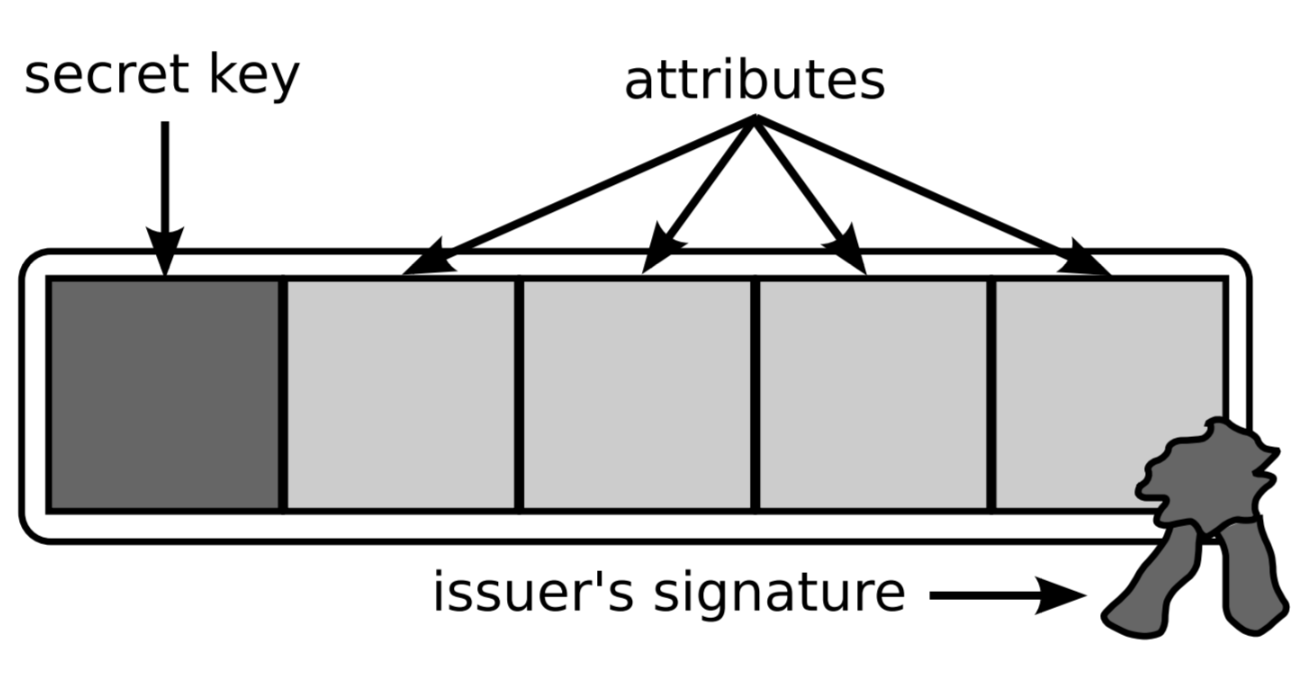
\includegraphics[width=0.4\linewidth]{gfx/ABC}
	\end{center}
	\caption{A first look at an attribute-based credential with four attributes.}
	\label{fig:abc}
\end{figure}



The Privacy Preserving Attribute Based Credentials system is composed by several actors, each one of them with different roles. One entity could act with more than one role, e.g., in a M2M (Machine To Machine) scenario, a device could act as both User and Verifier to other peers; but one can assume each actor acts with one role at a time.


The roles are:


\begin{figure}[bth]
	\begin{center}
		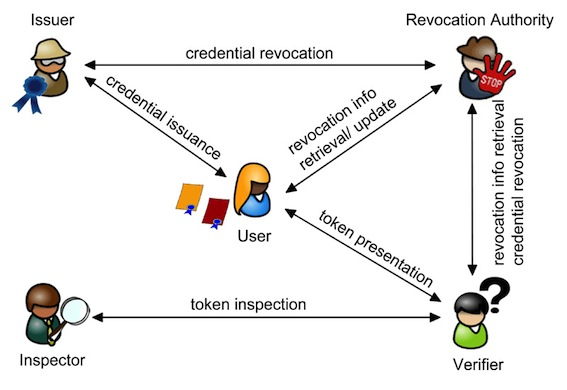
\includegraphics[width=\linewidth]{gfx/actors}
	\end{center}
	\caption{Entities in a P2ABC System}
	\label{fig:actors}
\end{figure}

\begin{itemize}
	\item \textbf{Issuer}\\
	In the ABC infrastructure, the Issuer is a trusted entity responsible for issuing credentials, vouching for the correctness of the information contained. Each Issuer generates a secret key and publishes the Issuer parameters that include the corresponding public verification key.
	
	\item \textbf{User}\\
	Entities that collect credentials from various Issuers. They can decide between all their credentials which attributes and values to present when making assertions about their identity to service providers.
	
	\item \textbf{Verifier}\\
	A service provider that protects access to a resource by imposing restrictions on the credentials that users must own and the information from these credentials that users must present in order to access the service.
	
	\item \textbf{Revocation Authority} (optional)\\
	This entity is responsible for revoking issued credential, preventing their further usage to generate a presentation token. Each revocation authority generates and publishes its revocation parameters.
	
	\item \textbf{Inspector} (optional)\\
	The Inspector's duty is to de-anonymize the user's presentation token under specific circumstances (e.g. misuse or liability). At setup, each inspector generates a private decryption key and a corresponding public encryption key. Usually, the capability of inspection should be bonded to privacy protection laws.
	
\end{itemize}

In our work, we aim at making IoT constrained devices capable to act as a User or Verifier in the P2ABCE architecture, given, for example, a M2M (Machine to Machine) setup, a device could identify itself to others (User), and ask for the respective cryptographic evidence to its peer (Verifier).


The key operations of Idemix are the Issuance and Proving, but there are also others like the revocation of credentials, update of attribute values or inspection of a prove. We consider that the cryptographic details of Idemix are out of the scope of this thesis, and can be consulted in \citep{idemixSpec}, but we will give a brief introduction of the Issuance and Proving interactions. Also, for those who want a little more information about the mathematical operations performed, without the deep explanations from the Idemix specification, we recommend to read the section 3.2 from \citep{vullers2013efficient}.


\hfil

The \textbf{Issuance} protocol consists on an interactive Camenisch - Lysyanskaya signature, that is, unlike usual signatures, where the Issuer alone hashes the credential (implying she knows all the values in it) and ciphers the digest, in this signature, the signing is performed between both actors.

This is possible given the nature of the CL signature, where the values of the parameters act as exponents of some public bases, and the use of ZKPs assure each party performs the correct calculations, avoiding malicious users. The User will perform the exponentiation with her secret key and some hidden attributes (the Issuer won't know their true value, only that they have some property, through a ZKP). The User then sends this new value and a ZKP that she indeed knows the exponents (the hidden values in the credential) for the public bases, without revealing said exponents. The Verifier performs the same exponentiation with the public attributes (not hidden by the User), and using her secret key, finishes the signature. The User then receives a valid CL signature for the credential, and no one except her knows the secret key and hidden values, thanks to the ZKPs.

The \textbf{Proving} protocol is simpler than the Issuance. It is usually performed in a three step protocol. First, the Verifier generates a nonce for the current interaction. Then, the User performs a non-interactive Zero-Knowledge Proof of any predicate she wants to proof. This is performed doing various ZKPs in parallel, using the same nonce from the Verifier. After the non-interactive ZKP is performed, the User sends it to the Verifier, which needs less calculations to verify the predicate, and learns nothing more than that the predicate itself is true, that is the nature of Zero-Knowledge Proofs.

Although we see both protocols are interactive, with at least 3 messages each, we mention \textit{non-interactive} ZKPs. If we recall the cave story, Victor needed to repeat the experiment many times before believing that Peggy knew the secret. Here, using the Fiat-Shamir heuristic and the Verifier nonce, the Verifier challenges (in the story, the path to return from) are substituted by a Hash function, e.g. SHA256, performed over some values. The User can't anticipate the digest result, so the Verifier trusts the Zero-Knowledge Proof, even when she doesn't choose the challenge. The Fiat-Shamir heuristic significantly increases the performance of these protocols, reducing the number of messages exchanged.



\hfil

As we have seen, Zero-Knowledge Proofs used in Idemix allow a user to prove ownership of a credential without
revealing the credential itself. Since the verifier does not see the credential, verification
instances are unlinkable and they also cannot be related to the issuing procedure. The privacy of users is protected by these unlinkability properties, even if the credential issuer and all verifiers collude. We can identify the following key features of the Idemix system \citep{vanet}:

\begin{itemize}
		
	\item \textbf{Issuance unlinkability}: the issuer cannot link an issued credential to the presentation of such credential.

	\item \textbf{Multi-show unlinkability}: a credential can be used multiple times without
	the resulting evidence becoming linkable.
	
	\item \textbf{Selective disclosure of attributes}: allows users to prove only a subset of
	attributes to a verifier.
	
	\item \textbf{Predicate proof}: it consists of statements that allow to prove a property
	of an attribute without disclosing its actual value. Example of these statements
	are the logical operators > or <.
	
	\item \textbf{Proof of holdership}: a cryptographic evidence for proving ownership or
	possession of a credential without disclosing the attributes contained in
	that credential.
	
	\item \textbf{Non-transferability}: key binding can be used to bind one or more credentials
	of a user to the same secret.
	
	\item \textbf{Scope-exclusive pseudonyms}: a certified pseudonym unique for a specific
	scope and secret key, i.e. a single pseudonym can be created for each credential.
	
	\item \textbf{Carry-over attributes}: it relies on the assumption that the user already
	possesses a credential, from which a given attribute can be carried over
	into the new credential without disclosing the attribute value to the Issuer.
	
	\item \textbf{Cross-credential proofs}: it allows users to prove relations between attributes
	from two or more credentials without revealing them to the verifier. For
	instance, that the name contained on a credit card and on a passport
	match.
	
	\item \textbf{De-anonymization}: it is an optional feature that allows an Inspector, either
	alone or in cooperation with other entities, to reveal the identity of users
	in cases of accountability and non-repudiation.
	
	\item \textbf{Revocation}: in case of misuse, it allows the revocation of issued credentials
	to (misbehaving) users. Thus, revoked credentials can no longer be used to
	generate Presentation Tokens.

\end{itemize}

To sum up, an attribute-based credential contains attribute-value pairs that are certified by a trusted Issuer. A credential can also specify one or more Revocation Authorities who are able to revoke the credential if necessary. Using her credentials, a User can form a presentation token that contains a subset of the certified attributes, provided that the corresponding credentials have not been revoked. Additionally, some of the attributes can be encoded in the presentation token so that they can only be retrieved by an Inspector. Receiving a presentation token from a User, a Verifier checks whether the presentation token is valid w.r.t. the relevant Issuers and Inspector's public keys and the latest revocation information. If the verification succeeds, the Verifier will be convinced that the attributes contained in the presentation token are vouched by the corresponding Issuers.


\hfil



\subsection{P2ABCE Code Structure and REST Services}


In the P2ABCE repository\footnote{\url{https://github.com/p2abcengine/p2abcengine}} there is available the project's code, divided in two solutions: a complete P2ABCE implementation in Java and a MULTOS smart card implementation as PoC for the project.


The Java code is managed by a Maven project, structured using various known design patterns, but this code is not our main target, as it won't be executed in the device. The part we are actually interested in are the \textit{REST Services} and their use of the \textit{Components} classes, where the smart card's logic and use are defined.

P2ABCE project is based on the concept of smart cards, virtual or physical, to store the Idemix credentials and keys. An interface is defined to communicate with these smart cards, and then different implementations allow to use either \textit{Software Smartcards} or \textit{Hardware Smartcards}. 

The \textit{SoftwareSmartcard} class implements the interface in Java, suitable for applications using P2ABCE self-storing digital smart cards, like a virtual wallet. This implementation is useful, for instance, to be deployed in more capable IoT devices (that can run Java) such as smartphones or smartwatches.

The \textit{HardwareSmartcard} class uses the standard APDU messages (\ref{subsec:APDU}) to interact with smartcards. P2ABCE defines the necessary APDU instructions for the smart card needed to implement each method of the interface. It relies on \texttt{javax.smartcardio} abstract classes (implemented by Oracle in their JRE) to communicate the smart card reader and the smart card. This way, it doesn't matter what manufacturer issues the smartcard, or if it's an Android device with NFC, if they support the APDU instructions, P2ABCE will work with them.

\begin{figure}[bth]
	\begin{center}
		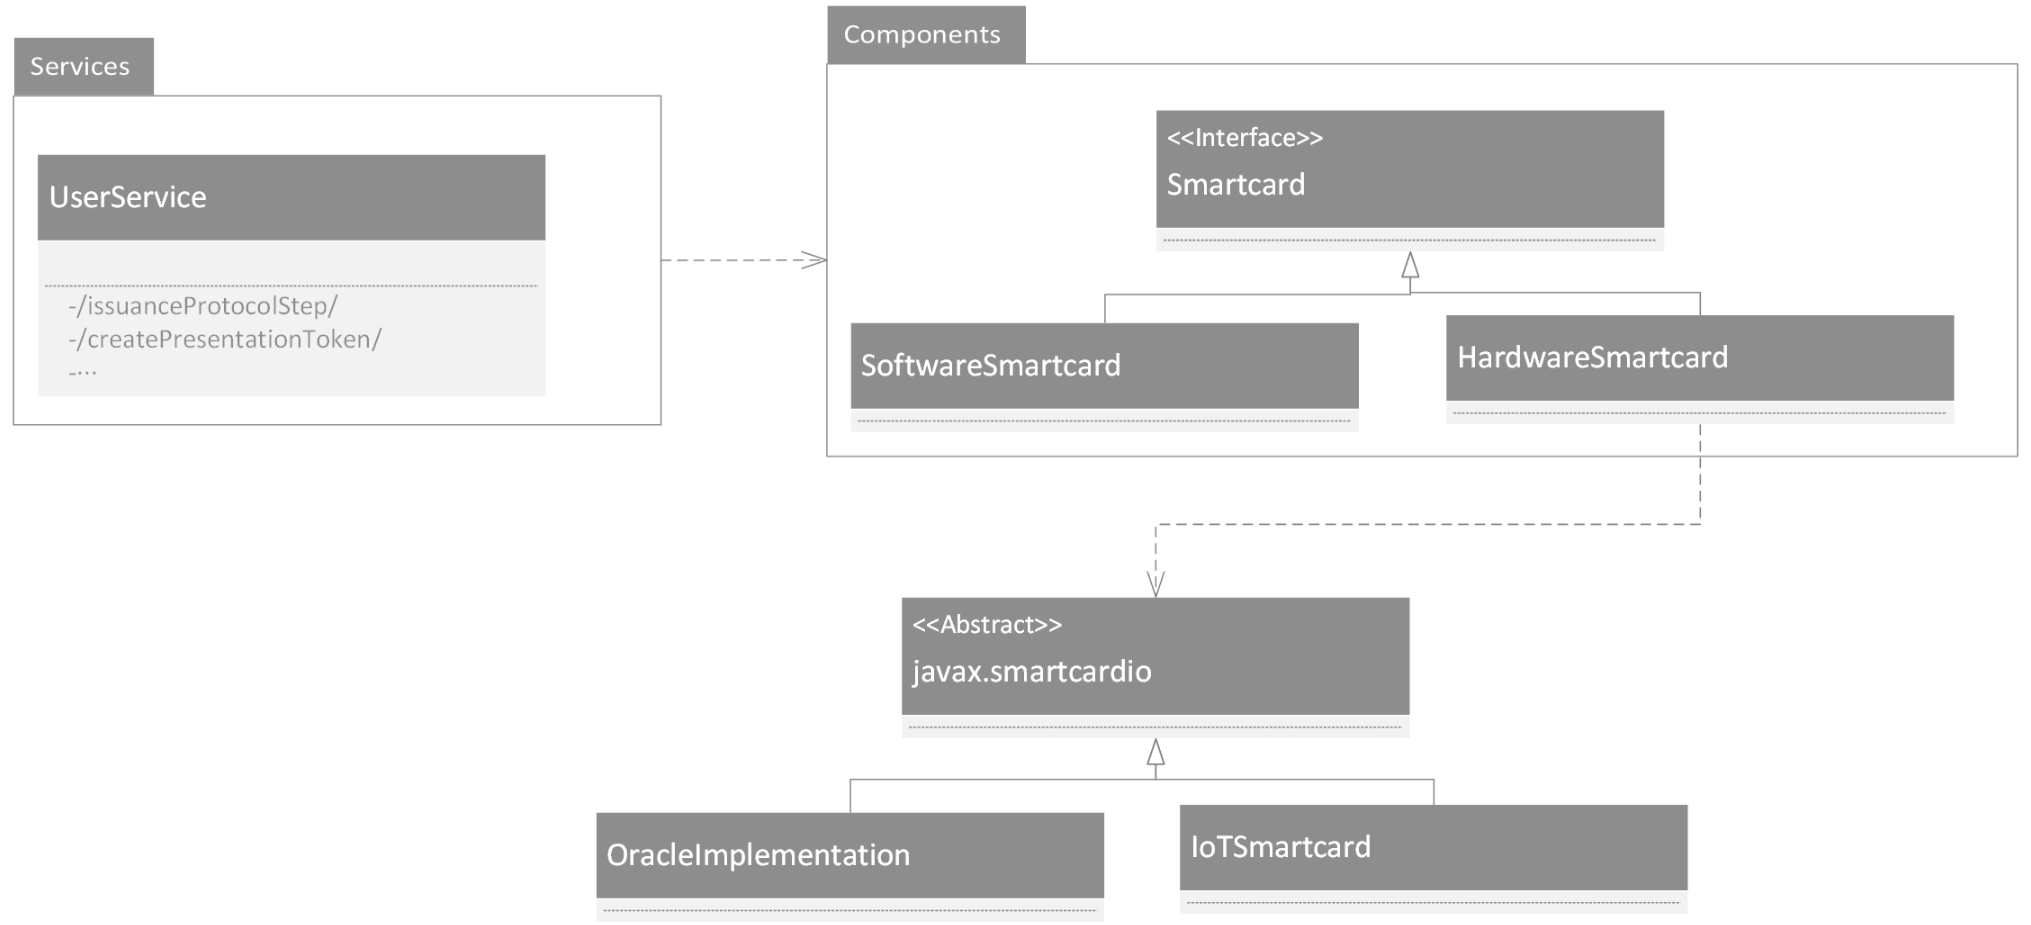
\includegraphics[width=\linewidth]{gfx/UML/p2abceBasicUML}
	\end{center}
	\caption{Basic P2ABCE structure}
	\label{fig:p2abceBasicUML}
\end{figure}


\hfil

The project also provides a set of REST services to control each role of the P2ABCE project (User, Issuer, Verifier, Inspector, etc.). The methods implemented include the creation of \textit{Software} smart cards within the User Service, and store them in a data base for future REST calls that may need them.

The services receive parameters like the length of the cryptographic keys, IDs, or XML files to parse. The REST API is not meant for a User Service to communicate with an Issuer Service or Verifier, but for the User actor to call the P2ABC Engine through the User Service, to perform specific actions (execute the User side of the Idemix issuance and proving protocols), and then this Service returns the Response XML. Those XML files are the way to communicate two different actors (e.g. User and Verifier). The transmission method to exchange the XML depends on the specific scenario.

This Services as \textit{tools} for the actors are only present in the P2ABCE project, not part of the Idemix or U-Prove engines. They are useful in a desktop environment, where we have a User Service in the background, and many programs, browser plugins, etc., make use of the Engine through the REST interface, reducing the number of P2ABCE entities in execution.


\subsection{ABC4Trust Card Lite}

As a PoC the P2ABCE project includes a smart card reference implementation, the ABC4Trust Card Lite \citep{ABC4TCardLite}. It supports device-bound U-Prove and Idemix, and virtually any discrete logarithm based pABC system.

Version 1.2 is written for \texttt{ML3-36K-R1} MULTOS smart cards, with approximately 64KB of EEPROM (non-volatile memory), 1KB of RAM and an Infineon SLE 78 microcontroller, a 16-bit based CPU aimed for chip cards.

The card stores the user's private key $x$ and any \ac{BLOB} that the P2ABCE may need (like user's credentials). Then P2ABCE delegates the cryptographic operations on the smart card, that operates with $x$.

\begin{figure}[bth]
	\begin{center}
		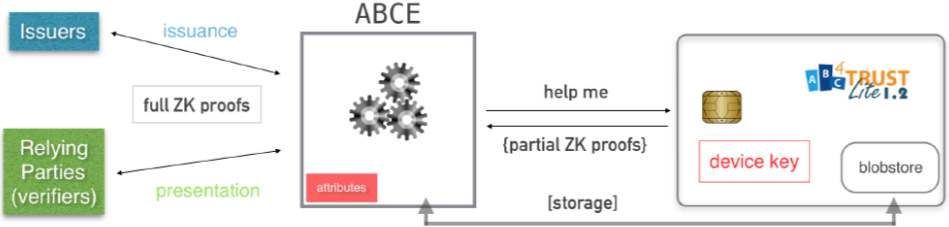
\includegraphics[width=\linewidth]{gfx/ABC4TCardLite}
	\end{center}
	\caption{ABC4Trust Card Lite. \textit{Image from ABC4Trust EU Project.}}
	\label{fig:ABC4TCardLite}
\end{figure}

The cryptographic operations performed by the smartcard are the modular exponentiation and addition used by ZKPs based on the discrete logarithm problem.

\hfil

The code is available from the P2ABCE's repository and has some good and bad points to take into account:

The best asset of this code is that it is written in C aiming to a very constrained device, with very limited memory and similar computational power to many other IoT devices.

The code uses some good practices when programming for constrained devices, also explained in the first implementation of Idemix in smart cards \citep{vullers2013efficient}. Aside the implementation in assembly code of some operations to accelerate the execution, most techniques aim to reduce the memory usage. They define \texttt{union} data types to join variables never used at the same time, so they can be stored on the same data location. Instead of function parameters, most variables are made global, reducing the space on the stack used when calling other functions. If parameters are needed, there are pointers to shared buffers with fixed sizes, avoiding the use of any dynamic memory allocation.


On the other side, among the many \textbf{drawbacks}, we could highlight the \textit{awful} coding style, the strong dependency on MULTOS framework and the fact that many bugs were found during our work.

The MULTOS C subroutines are an interface to hardware implementations for the smart cards, and it implies the ported code must be rewritten to an interoperable C code, not dependant on MULTOS specific functions.

The code is also affected by the MULTOS architecture, breaking many execution sequences, that is, the running application can stop at any point, not returning from a function. The MULTOS OS will read the public memory to generate a Response APDU and then clean the stack memory, but our standard C application must return from every function, freeing the used memory, minimizing possible errors from bad memory management. As we will see in the next chapter, the sequence diagram shows how any execution should perform, returning to the caller, not finishing the process when an error happens.

Although we mentioned the use of pointers as a way to reduce memory usage, we all agree that pointers are \textit{double–edged swords}, and a code with such an intense use of them is prone to undetectable errors before runtime.

The code is structured in two files, \textit{main.h} and \textit{main.c}, with around $550$ and $5200$ lines of code, respectively. The file \textit{main.h} is mostly a reimplementation in assembly MEL code of some MULTOS functionality already offered by their API.

The \textit{main.c} consists on nearly $600$ lines of variables and data structures declarations; followed by the \textit{main()} function, a $2600$ lines long \textit{switch-case} expression, that handles every APDU instruction, with practically no comments; and to conclude, the implementation of thirty functions called \textit{Subroutines} at the end of the file, with around other $2000$ lines of code.

\hfil

At this stage, we have two options to implement our IoT device compatible with P2ABCE:

\begin{itemize}
	\item Implement in C the \texttt{Smartcard} interface used by P2ABCE architecture, like the \texttt{SoftwareSmartcard} class, and use some communication protocol to remotely call the methods from the machine running the P2ABC Engine.
	\item Present the IoT device as a hardware smart card, using the APDU protocol (already defined, standard and with minimal overload). Providing a \textit{javax.smartcardio} ``IoT implementation'' to communicate with the IoT device through a transmission protocol, making the already existing \textit{HardwareSmartcard} class compatible with the new \textit{IoTSmartcard} running in the IoT device.
\end{itemize}

Even with the problematic to maintain or even understand the code of ABC4Trust Card Lite, once one studies MULTOS framework in deep, applies many refactoring techniques to the code, consider the applied optimizations for constrained devices, and the APDU protocol compatibility to work with \texttt{HardwareSmartcard} as any other smart card, it becomes the best starting point for the IoT version, making us opt for the second option.





\section{Preliminaries about smart cards}

We have decided to extend this chapter in order to explain the basis of smart card technologies, instead of only referencing the corresponding documentation, involving the reader to make the effort of understanding a system that is more complex than what we actually need to know at this point.

This section is a summary of the smart card's communication protocol, the MULTOS ecosystem, and, therefore, the inherited ABC4Trust Card Lite code, and how our IoT solution will work in the inside, acting as a smart card, a port from a (poorly coded) MULTOS application.


\subsection{Smart Card Communication Protocol}\label{subsec:APDU}

To communicate the smart cards and the reader the \texttt{ISO/IEC 7816-4} \citep{APDUISO} specifies a standardized protocol .

The messages, also kown as \acp{APDU}, are divided in APDU Commands and APDU Responses.

\textbf{APDU Commands} consist in 4 mandatory bytes (CLA, INS, P1, P2), and an optional payload.

\begin{itemize}
	\item CLA byte: Instruction class. Denotes if the command is interindustry standard or proprietary.
	\item INS byte: Instruction code. Indicates the specific command.
	\item P1, P2 bytes: Instruction parameters.
	\item Lc, 0-3 bytes: Command data length.
	\item Command data: Lc bytes of data.
	\item Le, 0-3 bytes: Expected response data length.
\end{itemize}

This way, minimal number of bytes are needed to transmit commands to the smart card, allowing manufacturer's personalization of the smart card behavior and capabilities along with standard operations.

\begin{figure}[bth]
	\begin{center}
		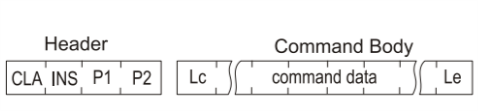
\includegraphics[width=0.55\linewidth]{gfx/APDUCommand}
	\end{center}
	\caption{APDU Command}
	\label{fig:APDUCommand}
\end{figure}


\textbf{APDU Responses} are generated inside the smart card, always as an answer to an APDU Command. They consist on an optional payload and two mandatory status bytes.


\begin{itemize}
	\item Response data: At most Le bytes of data.
	\item SW1-SW2 bytes: Status bytes. Encode the exit status of the instruction.
\end{itemize}

\begin{figure}[bth]
	\begin{center}
		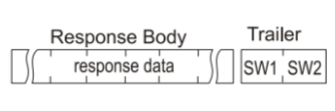
\includegraphics[width=0.55\linewidth]{gfx/APDUResponse}
	\end{center}
	\caption{APDU Response}
	\label{fig:APDUResponse}
\end{figure}




\hfil


The transmission protocol varies between different types of readers and smart cards (e.g. chip, contact-less), but what is common between every smart card interaction, is the \textit{APDU Command-Response Dialogue}. As long as the smart card has a power supply, it can maintain the memory in RAM between APDU Commands, what allows to do in two or more steps complex operations, transmit more bytes than a single APDU can admit, etc.

\hfil




\begin{figure}[bth]
	\begin{center}
		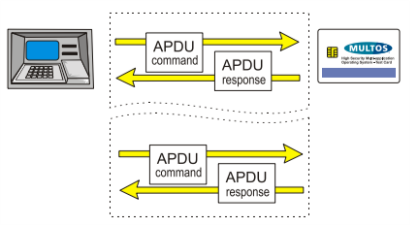
\includegraphics[width=0.75\linewidth]{gfx/APDUdialog}
	\end{center}
	\caption{APDU Command-Response Dialogue}
	\label{fig:APDUdialog}
\end{figure}

Originally, the Lc and Le bytes had only 1 byte, if present, restricting the payload data to be at most 256 bytes long. An extension to the protocol changed the meaning of a Lc or Le 0x00 byte (256 bytes long payload), so when the byte corresponding to Lc or Le started with 0x00, the next two bytes where the real length.  With this, an Extended APDU lets up to $65536$ bytes of data.

The problem here, is that not all readers or smart cards support extended APDUs. Originally, to send more than 256 bytes of data in an APDU Command, a \textit{Put Data} instruction is defined, so the smart card stores the payload in a buffer, until other APDU Command indicates how to use it.

To send more data in an APDU Response, the status bytes are set to: SW1=0x61 and SW2 to the remaining bytes to send. Because a smart card can't send APDU Commands, the card terminal must send a \texttt{GET RESPONSE}, a special APDU Command, with Le set to the number of bytes specified in SW2. Iterating this process, the smart card can send as many bytes as it wants as Response.

With the introduction of Extended APDUs, this technique is no longer needed.






\subsection{MULTOS}

MULTOS is a multi-application smart card operative system, which provides a custom developing environment, with rich documentation\footnote{MULTOS technical library - \url{http://www.multos.com/developer_centre/technical_library/}}. MULTOS smart cards communicate like any other smart card following the standard, but internally offers a very specific architecture, affecting the way one must code applications for it.

In this section we will present the main characteristics of a MULTOS smart card that shaped the ABC4Trust Card Lite code and that we had to be aware of when adapting it to IoT devices.


\paragraph{MULTOS programming languages} A native assembly language called MEL, C and, to a lesser extent, Java, are the available languages to code for MULTOS. In our case, ABC4T Card Lite uses MEL and C.

\paragraph{Execution Model}
Applications on a MULTOS card are executed in a virtual machine, called the Application Abstract Machine (AAM). The AAM is a stack machine that interprets instructions from the MULTOS Executable
Language (MEL).

The transmission and communication process is done by MULTOS core, and it then selects, based on the CLA byte of the APDU, the application to load. This application is what most developers will only worry about, and is where their compiled \texttt{main()} function will start.

\begin{figure}[bth]
	\begin{center}
		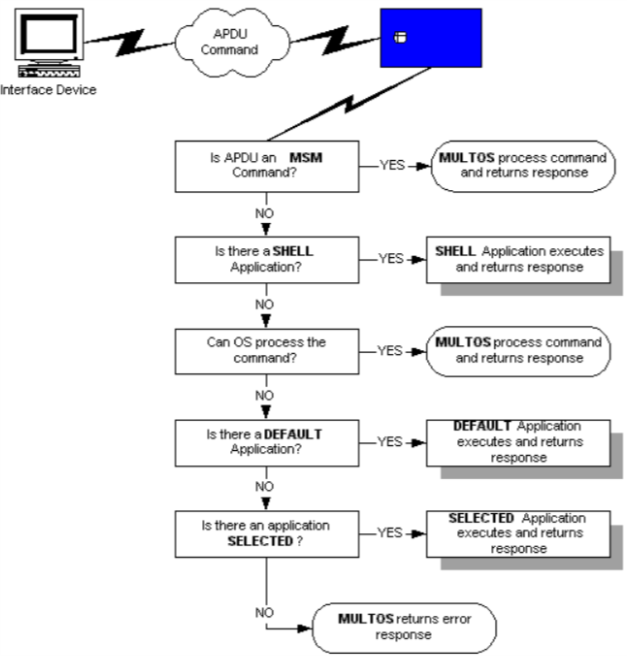
\includegraphics[width=0.6\linewidth]{gfx/multosWorkflow}
	\end{center}
	\caption{MULTOS Workflow}
	\label{fig:multosWorkflow}
\end{figure}

Now the developer is in charge of checking what instruction was sent, handle it with regard to his domain logic,  write in the specific data space the APDU Response bytes, and call \texttt{multosExit()}, a MULTOS API function that will be in charge to send the APDU Response.
In summary, our application starts with all data loaded in memory and exits without worrying how the answer is sent back.

As it can be sees, MULTOS is a comfortable framework to develop smart card applications, and now we must adapt and implement it for our IoT devices, if we want to port ABC4Trust Card Lite's code.



\paragraph{MULTOS Memory Layout}

Each application in MULTOS has access to a specific memory layout, divided in different categories:

\begin{figure}[bth]
	\begin{center}
		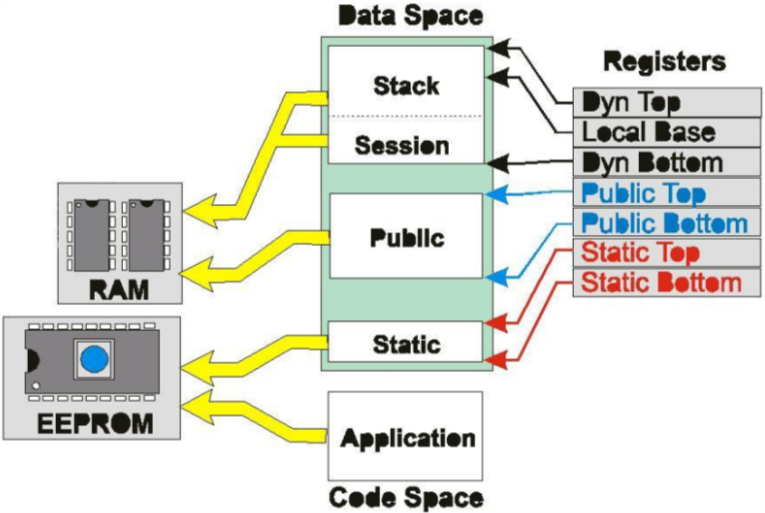
\includegraphics[width=0.8\linewidth]{gfx/multosMemLay}
	\end{center}
	\caption{MULTOS Memory Layout}
	\label{fig:multosMemLay}
\end{figure}


The Code Space is where the application code is stored.
The Data Space is divided in Static memory, Public memory and Dynamic memory.

\textbf{Static memory} are the application variables declared after the specific \texttt{\#pragma melstatic} compiler directive. These variables are stored in the non-volatile secure EEPROM, and any write is assured to be saved because they are not loaded into RAM.

\textbf{Public memory} can be seen as the input/output buffer for applications and MULTOS system. The APDU header appears at the top of Public, and command data at the bottom. The application writes then the APDU Response bytes in Public, at specific position (see \autoref{fig:multosPubMem}). To declare variables in this data space, the \texttt{\#pragma melpublic} directive is available.

\textbf{Dynamic memory} works like usual program memory, with Session Data storing global variables and the Stack. The limited size of RAM in IoT devices and smart cards makes the use of dynamic memory not advisable. The compiler directive to use Session Data is \texttt{\#pragma melsession}.


\begin{figure}[bth]
	\begin{center}
		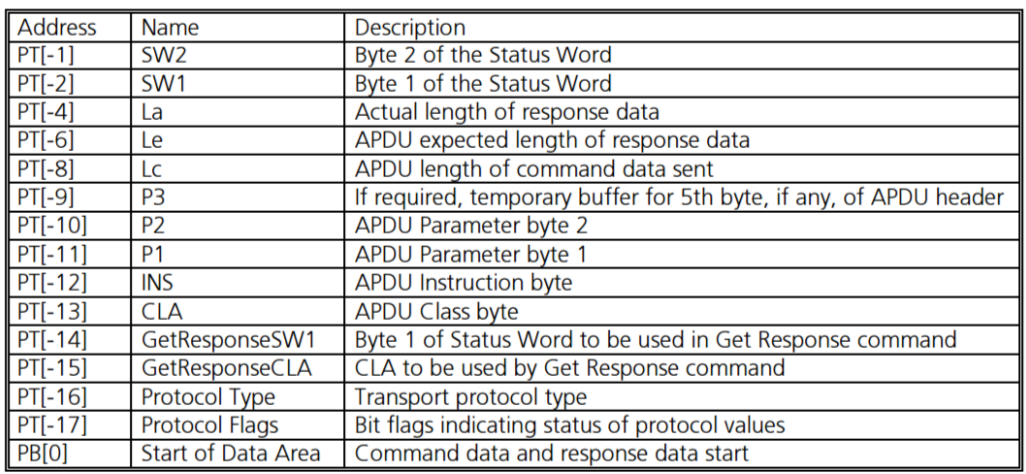
\includegraphics[width=\linewidth]{gfx/multosPubMem}
	\end{center}
	\caption{MULTOS Public Memory Data Map}
	\label{fig:multosPubMem}
\end{figure}


\hfil


With regards to primitive types, to avoid confusion with their sizes, MULTOS defines and uses the following data types specified in \autoref{fig:multosDataTypes}. It's important to notice that MULTOS is Big Endian
\marginpar{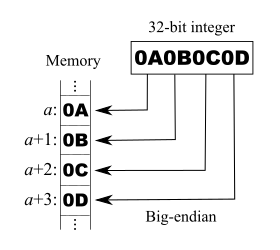
\includegraphics[width=\linewidth]{gfx/Big-Endian}\\Big-Endian, Wikipedia}
and when storing structures there is no padding between defined variables, unlike modern compilers that perform data structure alignment \footnote{\url{https://en.wikipedia.org/wiki/Data_structure_alignment}} for performance.

\begin{figure}[bth]
	\begin{center}
		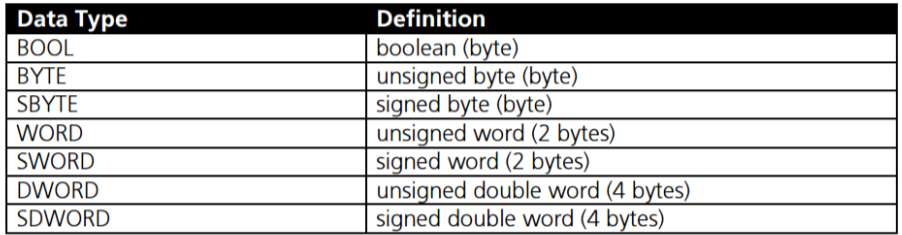
\includegraphics[width=\linewidth]{gfx/multosDataTypes}
	\end{center}
	\caption{MULTOS Data Types}
	\label{fig:multosDataTypes}
\end{figure}


\paragraph{MULTOS Standard C-API}

A collection of more than a hundred functions are provided for arithmetic, cryptography, memory and smart card operations. The \textit{multos.h} interface provides access to these functions, that ultimately call their respective primitive instructions in assembly code. The primitive instructions are but a system call with an operation code, loading data in the needed registers, and hardware implemented functionality. Therefore,  no implementation for these tools is available, nor in C, nor in assembly code.

Nevertheless, the C-API documentation\footnote{\url{http://www.multos.com/developer_centre/technical_library/}} provides rich description for each function.

Following this documentation, we will have to reimplement in C the same or extended functionality, trying to be as efficient as the hardware implementations in MULTOS smart cards. For example, the cryptographic operations are common in smart cards and therefore hardware supported, but a constrained IoT device does not usually include a cryptographic chip or specialized processor instructions.



\hfil

\section{Development environment}


For almost every IoT device in the market, there exists a C compiler and many frameworks available to build firmware binaries, like Arduino Core, Contiki, Mongoose OS, ThreadX OS, OpenWrt, LEDE, proprietary SDKs, etc. Each firmware targets a specific range of devices, depending on processing power and memory limitations. For example, Arduino and Contiki aim for very constrained microcontrollers, like Atmel's ATmega or TI's MSP430, but can also be used in ESP8266, a more powerful device, with WiFi capabilities.
\marginpar{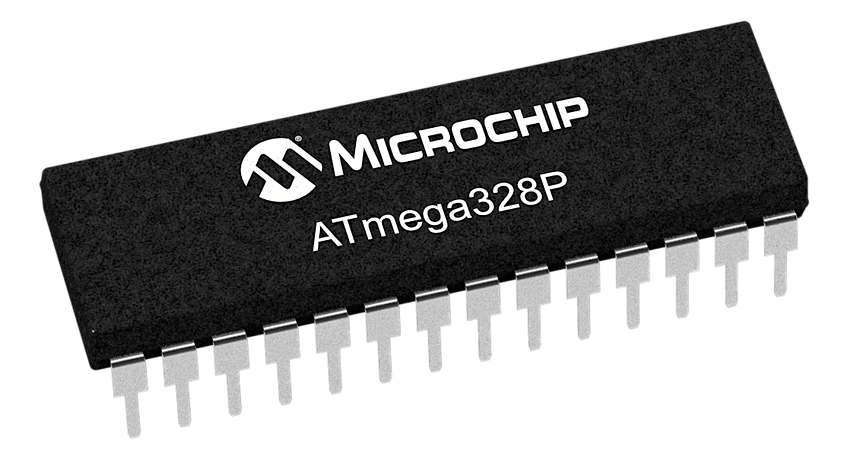
\includegraphics[width=0.8\linewidth]{gfx/ATmega328P}\\$ATmega328P$}

Starting a big project development for \ac{IoT}, aiming the most constrained devices may not be a good idea. The lack of usual OS tools, like POSIX, threads, or minimum I/O, like a terminal, can make debugging a tedious task. With good programming practices, one can start from the top and slowly end with more constrained devices and reliable code.


For this reason, the current \ac{PoC} is developed on LEDE\footnote{Linux Embedded Development Environment - \url{https://lede-project.org/}} using the Onion Omega2 development board. Although the Omega2 uses LEDE, its microcontroller is also listed as compatible with ThreadX\footnote{THREADX Real-Time Operative System for embedded devices - \url{http://rtos.com/products/threadx/}}, therefore, the performance measured in our PoC can be relevant to real scenarios with similar hardware.

The PoC will take advantage of the Linux system using mainly files and sockets like in any other Linux desktop distribution, so we can focus on the project itself rather than the specific platform APIs for storage and connectivity.


\hfil

The project development is divided between the IoT device code and the P2ABCE services. To ease the setup of new developing machines, we will use Docker\footnote{\url{https://www.docker.com/what-docker}} to deploy two containers, one ready to cross-compile our IoT project's C code, and the other container will compile the P2ABCE's Java code.

\hfil

P2ABCE is already written in Java and uses Maven to manage dependencies. The project needs some minor changes to work with our IoT architecture. Any text editor or Java IDE is suitable for the development, because the compilation is done through the terminal, with Maven commands.

We compile the project inside a Docker container, with OpenJDK 7, Maven 3 and Idemix 3.0.36, following the project \href{https://github.com/p2abcengine/p2abcengine/wiki/How-to-Build-the-ABC-Engine}{instructions} to use Idemix as the Engine for P2ABCE.

\hfil

We can assume all IoT devices have a C cross-compiler, some even a C++ cross-compiler. The worst case scenario is that one must write assembly code, and that code will be specific of that target, so we won't consider them.
If now we focus on the most constrained devices, we could find out that for some we can't use C++, some may not have many usual libraries, moreover, the memory limitations they face make practically impossible to use dynamic memory, if we want to avoid many execution malfunctions.

For that reason, the developed code for IoT devices should be written with standard C, without using dynamic memory or third party libraries.

\hfil


To manage the PoC code we chose CMake, providing many advantages over Makefiles:

\begin{itemize}
	\item Cross-platform. It works in many systems, and more specifically, in Linux it generates Makefiles.
	\item Simpler syntax. Adding a library, files to compile, set definitions, etc. can be done with one CMake command, with rich documentation on the project's \href{https://cmake.org/cmake/help/latest/}{website}.
	\item Cross-compilation. With only a \href{http://www.vtk.org/Wiki/CMake_Cross_Compiling#The_toolchain_file}{\small{CMAKE TOOLCHAIN}} file, CMake sets up automatically the cross-compilation with Makefiles and the C/C++ cross-compiler provided.
\end{itemize}


\hfil

Although the ideal final code is written in pure C, without external libraries or dynamic memory, the PoC uses three major libraries:

\begin{itemize}
	\item OpenSSL: Provides reliable and tested AES128, SHA256 and random number generator implementations.
	\item LibGMP: Provides multiprecision integer modular arithmetic.
	\item cJSON: Provides a JSON parser to store and read the status of the device, in a human readable way.
\end{itemize}

These three libraries are used to implement different interfaces in the project, and C implementations of these interfaces should replace the external libraries in the future.

\hfil

Finally, we use Docker to deploy the compilation environment. Our container includes CMake and the LEDE SDK \citep{ledeproject}, configured for the Omega2 target, the device chose for the PoC.


